\section{Weighted Graphs}
\subsection*{Dijkstra's}
Finds the shortest path from a src vertex to all other vertices in a weighted
directed graph w/out negative edge weights. (uses BFS)

\subsubsection*{Dijkstra's Trace}

\resizebox{.5\linewidth}{!}{%
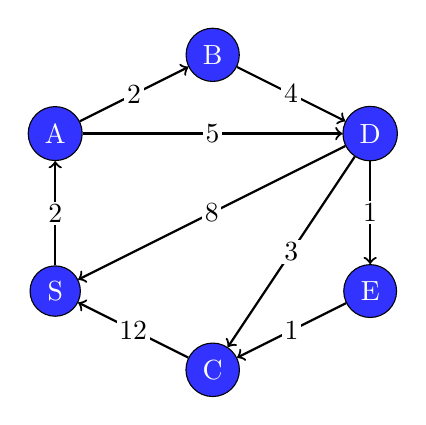
\begin{tikzpicture}[
    n/.style ={
        circle,
        white,
        fill=blue!80,
        draw=black
    },
    inside/.style ={
        midway,
        fill=white,
        inner sep=1pt,
        outer sep=1pt
    }
    ]
    \foreach \x/ \pos in {{A/(0,2)}, {B/(2,3)}, {C/(2,-1)}, {D/(4,2)}, {E/(4,0)},
                          {S/(0,0)}}
        \node[n] (\x) at \pos {\x};

    \foreach \src/ \dst/ \weight in {S/A/2, A/B/2, B/D/4, A/D/5, D/S/8, D/C/3, D/E/1, E/C/1, C/S/12}
        \draw[->,thick] (\src) -- node[inside] {\weight} (\dst);
\end{tikzpicture}
}

\begin{tabular}{@{} ccccccc @{}}
     & \multicolumn{6}{c}{Distances}\\
    {\scriptsize processed} & S & A & B & C & D & E\\
    \toprule
      & 0 & $\infty$ & $\infty$ & $\infty$ & $\infty$ & $\infty$ \\
    S (0) & 0 & 2 & $\infty$ & 12 & 8 & $\infty$ \\
    A (2) & 0 & 2 & 4 & 12 & 7 & $\infty$ \\
    B (4) & 0 & 2 & 4 & 12 & 7 & $\infty$ \\
    D (7) & 0 & 2 & 4 & 10 & 7 & 8\\
    E (8) & 0 & 2 & 4 & 9 & 7 & 8\\
    C (9) & 0 & 2 & 4 & 9 & 7 & 8
\end{tabular}

\subsection*{Minimum Spanning Trees}

\bold{tree:} A connected graph w/out cycles.

\bold{Spanning Tree:} A subtree of a graph that includes each vertex of the graph.
A subtree of a given graph as a subset of the components of that given graph.

\bold{Minimum Spanning Tree:} Only def for weighted graphs.
This is the spanning tree of a given graph whose $\sum\text{edge weights}$ is min, compared
to all other spanning trees.

%\vspace{1em}! % Fixes clipping issue with "min span tree" par


\resizebox{\linewidth}{!}{%
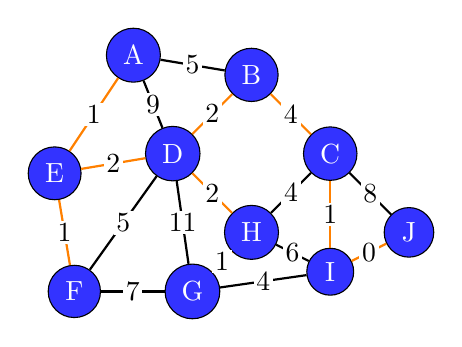
\begin{tikzpicture}[
    n/.style ={
        circle,
        white,
        fill=blue!80,
        draw=black
    },
    inside/.style ={
        midway,
        fill=white,
        inner sep=1pt,
        outer sep=1pt
    }
    ]
    \foreach \x/ \pos/ \sel in {{A/(1,3)/black}, {B/(2.5,2.75)/black}, {C/(3.5,1.75)/black}, {D/(1.5,1.75)/black},
                                {E/(0,1.5)/black}, {F/(0.25,0)/black}, {G/(1.75,0)/black}, {H/(2.5,0.75)/black},
                                {I/(3.5,0.25)/black}, {J/(4.5,0.75)/black}}
        \node[n] (\x) at \pos {\x};

    \foreach \src/ \dst/ \weight/ \sel in {E/F/1/orange, E/A/1/orange, E/D/2/orange, F/D/5/black, A/D/9/black, A/B/5/black,
                                     D/B/2/orange, F/G/7/black, G/D/11/black, G/H/1/orange, G/I/4/black, D/H/2/orange,
                                     H/I/6/black, H/C/4/black, B/C/4/orange, C/J/8/black, I/C/1/orange, I/J/0/orange}
        \draw[draw,thick,\sel] (\src) -- node[inside] {\color{black}\weight} (\dst);
\end{tikzpicture}
}
{\scriptsize ({\color{orange}orange}) Minimum spanning tree with weight 14}

\subsection*{Kruskal's}
\begin{enumerate}
    \item Sort edges by ascending edge weight.
    \item Walk through the sorted edges and look at the two nodes the edge belongs
        to, if the nodes are already unified we don't include this edge, otherwise
        we include it and unify the nodes.
    \item The algorithm terminates when every edge has been processe or all the vertices
        have been unified.
\end{enumerate}

%Let $V=\emptyset$

%For $i=1\to n-1$, (where there are n vertices in a graph)

%$V=V\cup e$, where $e$ is the edge w/ the min edge weight $\notin V$, and that does NOT form a
%cycle when added to $V$.

%Return $V$

\subsection*{Prim's}

A greedy MST algorithm that works well on dense graphs.
However, when finding the minimum spanning forest on a disconnected graph,
Prim's must be run on each connected component individually.

The lazy version of Prim's has a runtime of $O(E\log E)$, and the eager version
has a better runtime of $O(E\log V)$.

\subsubsection*{Lazy Prim's}

\begin{enumerate}
    \item Maintain a min Priority Queue that sorts edged based on min edge cost.
    \item Start the algorithm on any node \bold{s}. Mark \bold{s} as visited and iterate
        over all edges of \bold{s}, adding them to the PQ.
    \item While the PQ is not empty and a MST has not been formed, dequeue the next cheapest
        edge from the PQ.
        If the dequeued edge has already been visited, skip it and poll again.
        Otherwise, marked the current node as visited and add the selected edge to the MST.
    \item Iterate over the new current node's edges and all all its edges to the PQ.
        Do not add edges to the PQ which point to already visited nodes.
\end{enumerate}

\begin{lstlisting}[language=Java,basicstyle=\tiny]
// edge implements Comparable
public ArrayList<edge> prims(
  ArrayList<edge>[] graph
) {
  int n = graph.length;
  // shortened to PQ for spacing
  PQ<edge> pq = new PriorityQueue<edge>();
  boolean[] used = new boolean[n];
  used[0] = true;
  for (edge e: graph[0])
    pq.offer(e);

  ArrayList<edge> mst = new ArrayList<edge>();
  while (pq.size() > 0 && mst.size() < n-1) {
    edge cur = pq.poll();
    if (used[cur.u] && used[cur.v]) continue;
    int newV = !used[cur.u] ? cur.u : cur.v;
    mst.add(cur);

    used[newV] = true;
    for (edge e: graph[newV])
      pq.offer(e);
  }
  if (mst.size() < n-1) return null;
  return mst;
}
\end{lstlisting}

%\begin{enumerate}
    %\item Set $S=\emptyset$.
    %\item Pick any vertex in the graph.
    %\item Add the min edge incident to that vertex to S.
    %\item Continue to add edges into S (n-2 more times) using the following rule:
        %Add the min edge weight to S that is incident to S but that doesn't form
        %a cycle when added to S.
%\end{enumerate}

\subsection*{Network Flow}

\bold{Max-Flow, Min-Cut Theorem:} The value of the maximal flow in a flow network
equals the value of the minimum cut.

\subsubsection*{Ford Fulkerson}
While there exists an augmenting path:
Add the appropriate flow to that augmenting path.

Typically, DFS is used to check for the existence of an augmenting path.

worse-case, the algorithm takes $O(|f|E)$ time, where $|f|$ is the maximal flow  of the network.

\subsubsection*{Edmonds Karp Algorithm}
A variation on the Ford-Fulkerson method. Idea is to stry to choose good augmenting paths.
In this algorithm, the augmenting path suggested is the augmenting path with the mininal
number of edges. (Can be found using BFS) The total number of iters is $O(VE)$. Thus,
total run time with the graph stored as an adj.\ matrix is $O(V^3E)$.


\subsubsection*{Dinic's Algorithm}
A strongly polynomial max flow algorithm with a runtime of $O(V^2E)$.

The strongly polynomial means that the runtime does not depend on the capacity
values of the flow graph.

Extremely fast and works even better on bipartite graphs, with a time complexity
of $O(\sqrt{V}E)$ due to the algorithm's reduction to Hopcroft-Karp.

The main idea is to guide augmenting paths from $s\to t$ using a level graph.

\subsubsection*{Level Graph}

An edge is only part of the level graph if it makes progress towards the sink.
That is, the edge must go from a node at Level $L$ to another at level $L+1$.

\resizebox{\linewidth}{!}{%
\begin{tikzpicture}[
    auto,
    scale=2,
    n/.style ={
        circle,
        white,
        fill=blue!80,
        draw=black
    },
    inside/.style ={
        midway,
        fill=white,
        inner sep=1pt,
        outer sep=1pt
    }
    ]
    \foreach \x/ \y/ \pos/ \clr in {{S//(0,1)/orange}, {1/0/(1,0)/red}, {1/1/(1,1)/red}, {1/2/(1,2)/red},
                                {2/0/(2,0)/codegreen}, {2/1/(2,1)/codegreen}, {2/2/(2,2)/codegreen},
                                {3/0/(3,0)/purple}, {3/1/(3,1)/purple}, {3/2/(3,2)/purple}, {T//(4,1)/pink}}
        \node[n,fill=\clr] (\x\y) at \pos {\x\y};

    \foreach \src/ \dst/ \fwd/ \bck in {
        S/10/{0/15}/{0/0}, S/11/{0/10}/{0/0}, S/12/{0/5}/{0/0}, 11/12/{0/15}/{0/0},
        21/10/{0/5}/{0/0}, 10/20/{0/25}/{0/0}, 11/21/{0/20}/{0/0}, 12/22/{0/10}/{0/0},
        22/21/{0/25}/{0/0}, 31/22/{0/15}/{0/0}, 22/32/{0/10}/{0/0}, 21/31/{0/30}/{0/0},
        20/30/{0/10}/{0/0}, 20/31/{0/20}/{0/0}, 31/30/{0/10}/{0/0}, 32/T/{0/5}/{0/0},
        31/T/{0/15}/{0/0}, 30/T/{0/10}/{0/0}}{
        \path[->,dashed] let \p1=($(\src)-(\dst)$), \n1={atan2(\y1, \x1)}, \n2={180+\n1} in
            ($ (\dst.\n1)!1pt!90:(\src.\n2) $) edge node {\tiny \bck} ($ (\src.\n2)!1pt!-90:(\dst.\n1) $);
        \path[->] let \p1=($(\dst)-(\src)$), \n1={atan2(\y1, \x1)}, \n2={180+\n1} in
            ($ (\src.\n1)!1pt!90:(\dst.\n2) $) edge node {\tiny \fwd} ($ (\dst.\n2)!1pt!-90:(\src.\n1) $);
        %\draw[<->,thick] (\src) -- (\dst);
    };
\end{tikzpicture}
}

% TODO: Finish example: https://youtu.be/M6cm8UeeziI?t=347

Algorithm Steps:

\begin{enumerate}
    \item Construct a level graph by doing a BFS from the src to label all the levels
        of the current flow graph.
    \item If the sink was never reached while building the level graph, then stop and
        return the max flow.
    \item Using only valid edges in the level graph, do multiple DFSs from $s\to t$ until a
        blocking flow is reached, and sum over the bottleneck values of all the
        augmenting paths found to calculate the max flow.
    \item Repeat Steps $1\to 3$
\end{enumerate}

% If have room, may add Bipartite Matching:
% http://www.cs.ucf.edu/~dmarino/ucf/cop3503/lectures/NetworkFlow.pdf#page=7
